\section{Logical view}

Som beskrevet i view beskrivelser på forrige side består logical viewet af designoverview-, sekvens-, statemachines og klassediagrammer. Til at lave diagrammerne anvendes applikationsmodellen.

\subsection{Applikationsmodel}
Applikationsmodellen anvendes til at udvikle diagrammerne tilhørende logical view. Med applikationsmodellen tages der udgangspunkt i use cases beskrevet i kravspecifikationen og domain modellen, se figur \ref{fig:domain_model}.
  
Ud fra domain modellen identificeres de overordnede klasser der skal bruges til de forskellige use cases. Når de overordnede klasser er identificeret beskrives hvordan de kommunikerer via desginoverview og sekvensdiagrammer. Herefter laves statemachines med de fundne klasser og til sidst udarbejdes klassediagrammer.


\subsection{Iteration \#1}

\subsubsection*{User story}

Bruger tænder dronen ved at tilslutte batteri. Main controller samt 3G/GPS module initialiseres og nuværende GPS position opdateres. Herefter oprettes forbindelse mellem drone og webapplikation, og information om dronen er online samt information om dronens nuværende GPS position sendes fra dronen til webapplikation. Fra webapplikationen er det muligt for bruger løbende at observere hvorvidt dronen er online og på hvilken GPS position dronen befinder sig.

%kommentar
\begin{figure}[H]
	\centering
	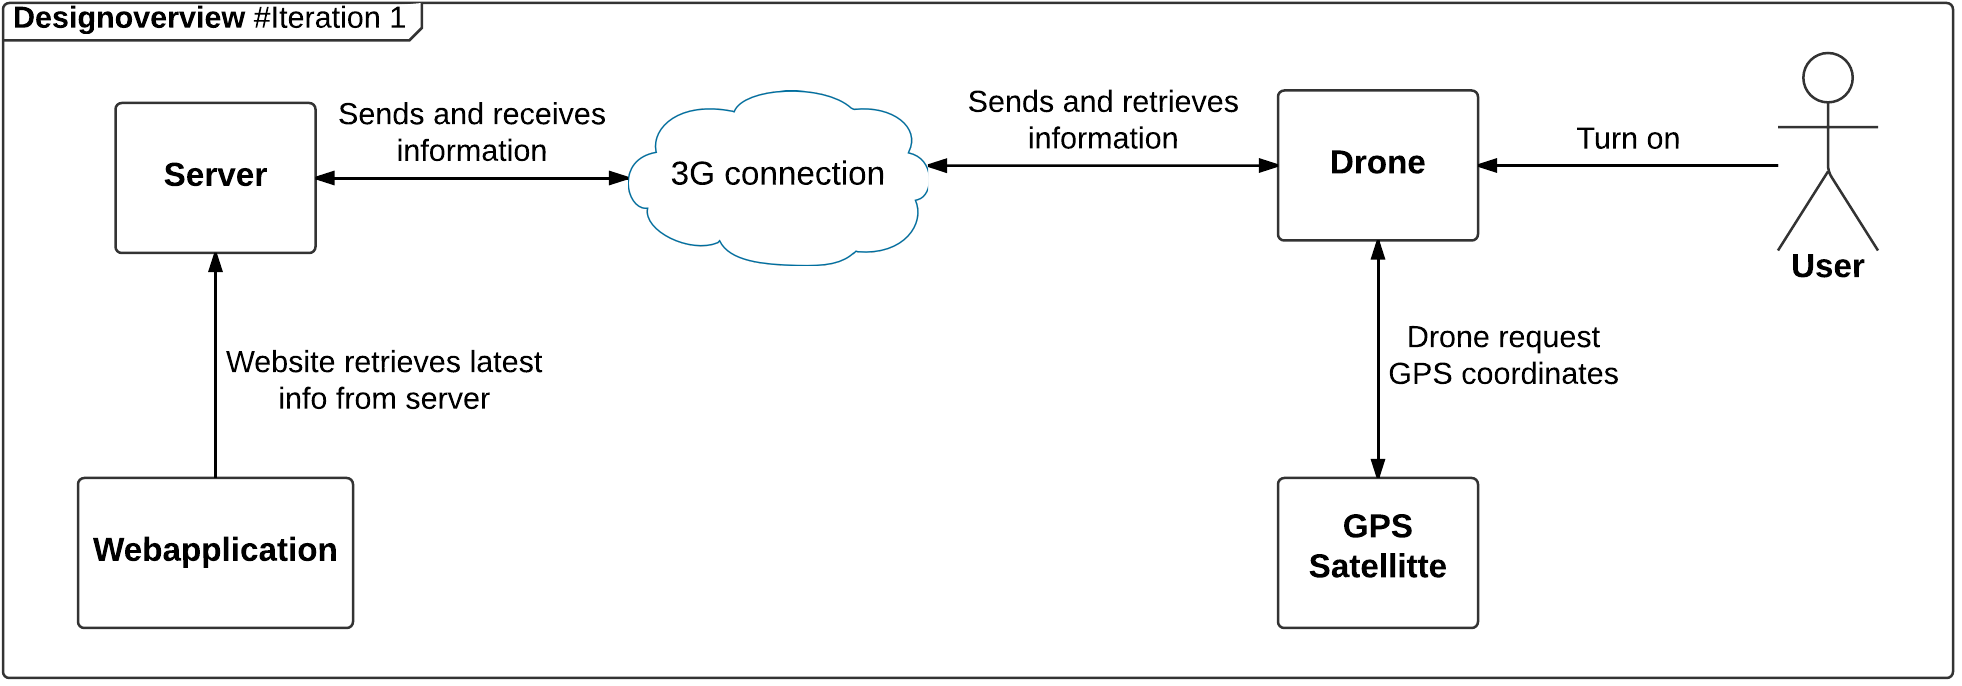
\includegraphics[width=1\textwidth]{Billeder/design_overview/design_overview_iteration1.png}
	\vspace{-.5cm}
	\caption{Design overview \#iteration 1}
	\label{fig:design_overview_UC1}
\end{figure}


\newpage
\subsubsection*{Sekvens diagram}
På sekvensdiagrammet på figur \ref{fig:Sekvens_diagram_iteration1}, vises hvilke klasser der indgår og bruges i første iteration. Af sekvensdiagrammet fremgår det, at sekvensen først startes når bruger tilslutter batteri og tænder dronen. Når der er tilkoblet forsyning initialiseres main controller samt 3G/GPS og nuværende GPS position  (longitude og latitude) opdateres. Dronens nuværende GPS position opdateres når dronen sender PUT requests til webapplikation. PUT requests bruges dels til at fortælle webapplikationen at dronen er online og dels til at give webapplikation information om dronens nuværende position. 


%kommentar
\begin{figure}[H]
	\centering
	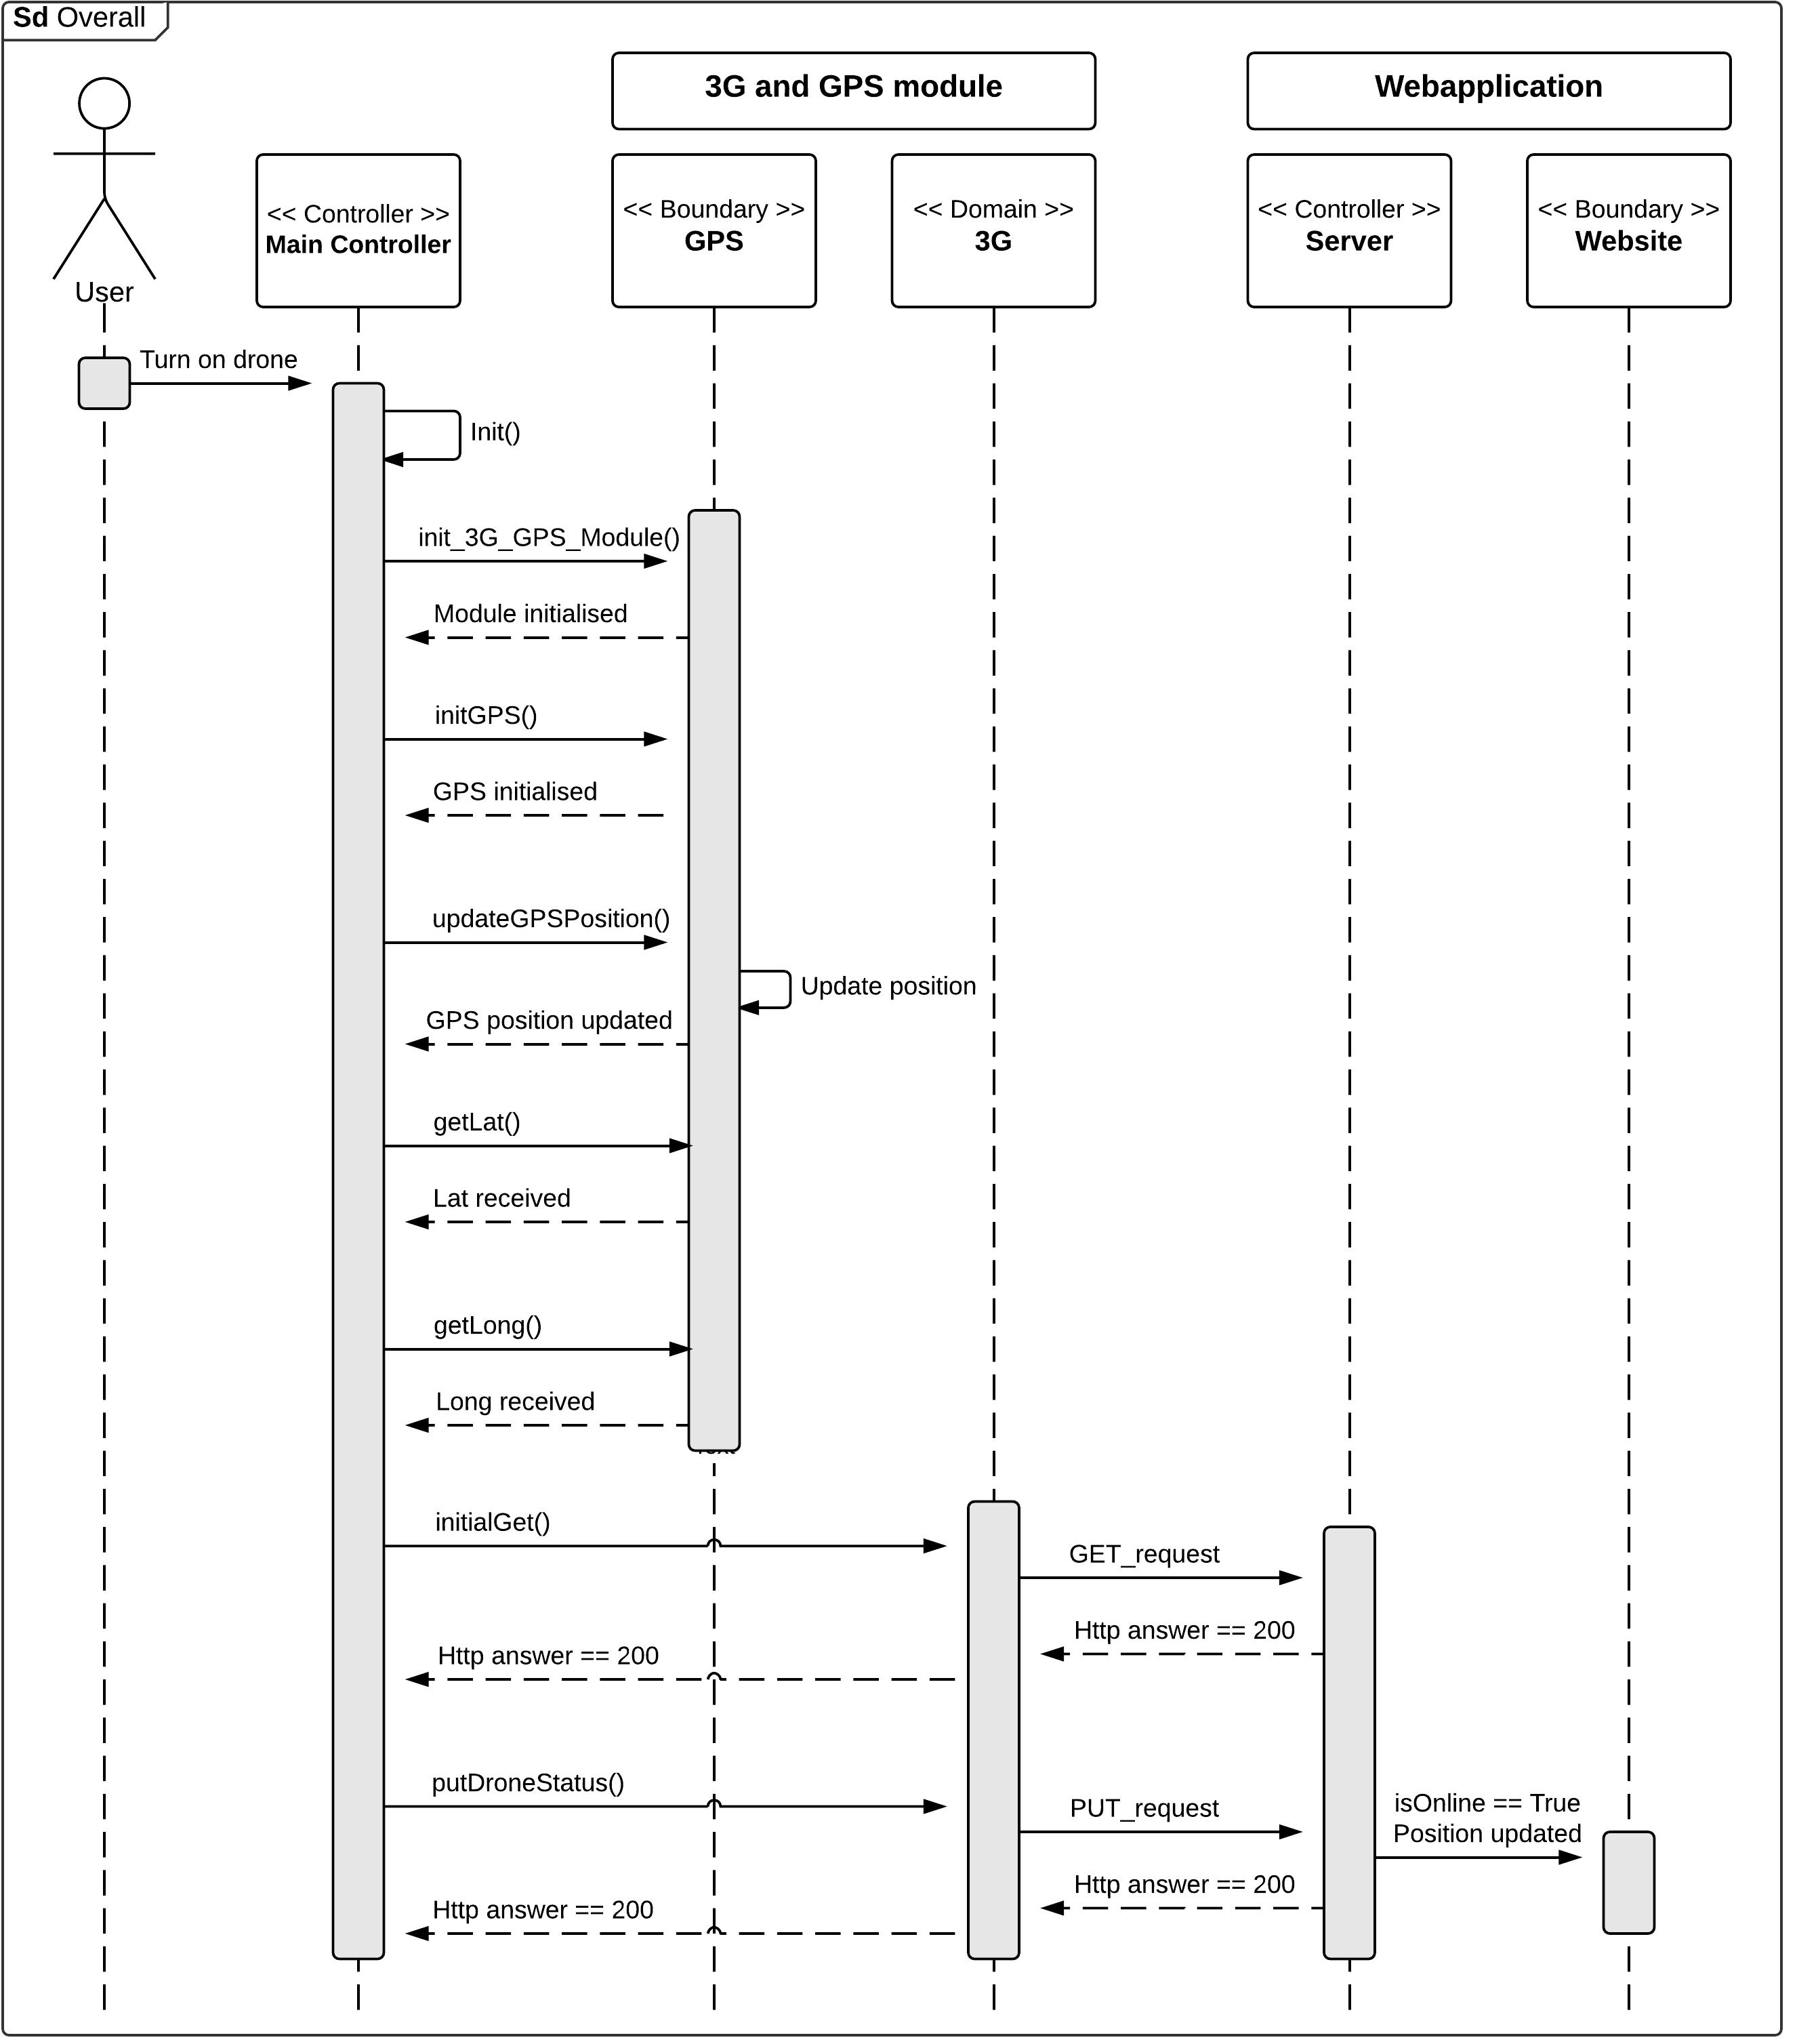
\includegraphics[width=0.93\textwidth]{Billeder/sekvens/sekvens_iteration1}
	\caption{Sekvens diagram \#iteration 1}
	\label{fig:Sekvens_diagram_iteration1}
\end{figure}

\newpage
\subsubsection*{State machine diagram}
I state machinen diagrammet figur \ref{fig:Statemachine_iteration1}, vises de forskellige states der eksisterer i iteration 1 og hvordan flowet imellem dem ser ud.
%kommentar
\begin{figure}[H]
	\centering
	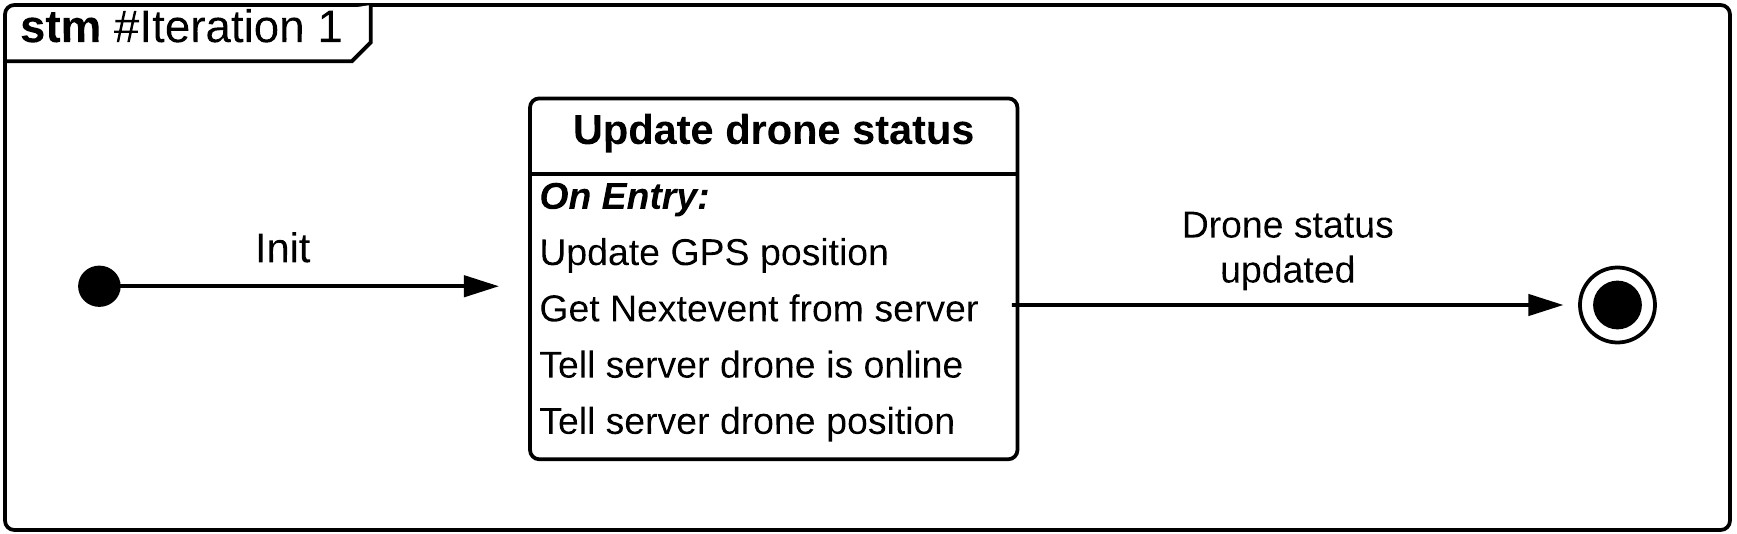
\includegraphics[width=1\textwidth]{Billeder/statemachine/State_iteration1.png}
	\vspace{-0.5cm}
	\caption{Statemachine \#iteration 1}
	\label{fig:Statemachine_iteration1}
\end{figure}

\subsubsection*{Klasse diagram}
Fint og flot klasse diagram ses nedenfor:
%kommentar
\begin{figure}[H]
	\centering
	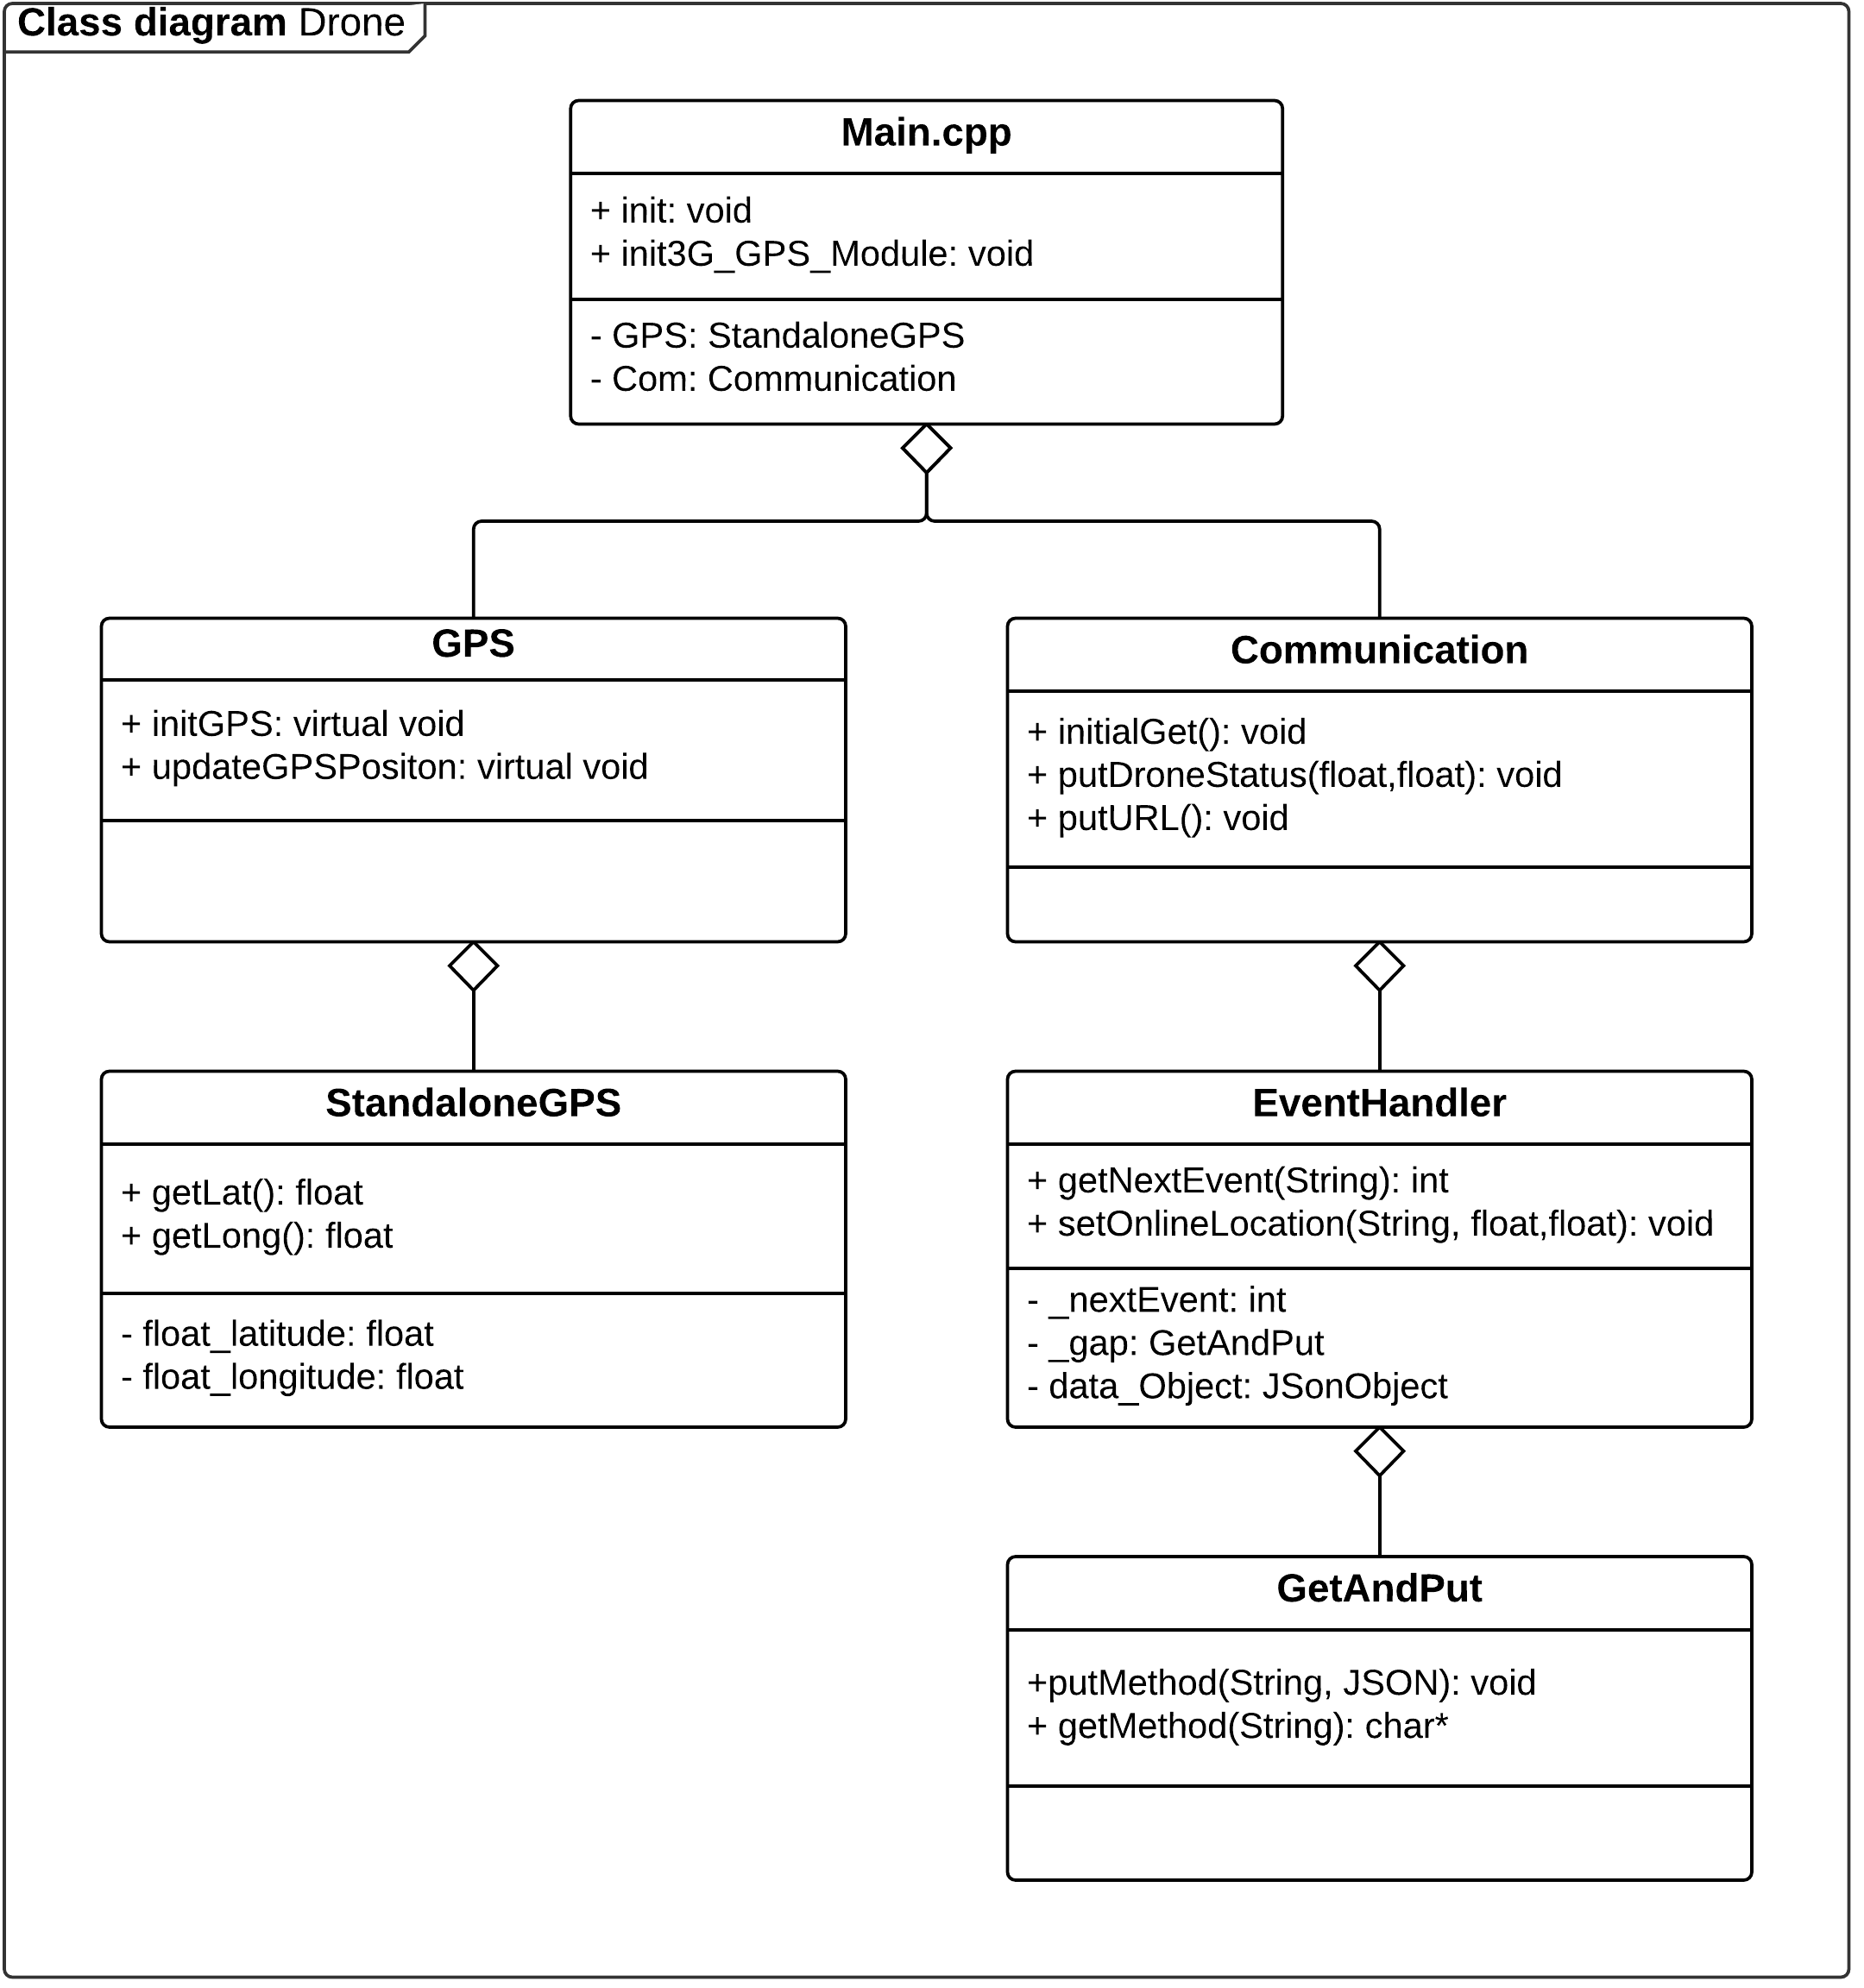
\includegraphics[width=1\textwidth]{Billeder/klasse_diagrammer/classdiagram_iteration1.png}
	\vspace{-0.5cm}
	\caption{Klassediagram \#iteration 1}
	\label{fig:Statemachine_iteration1}
\end{figure}

\newpage

\textbf{Main.cpp} \\
Main.cpp filen bruges til at sætte arduino board korrekt op, bla. sættes baudrate på de forskellige serielle forbindelser. Desuden bruges Main.cpp til at kalde og eksekverer forskellige klasse, objekter og funktioner.

\textbf{GPS} \\
GPS klassen fungerer som en virtuel klasse, og sikre som minimum implementering af init og updateGPSPosition uanset hvilken GPS der bruges. Klassen er lavet fordi der i udgangspunkt var mulighed for at bruge 3 forskellige slags GPS med 3G/GPS shieldet. 

\textbf{StandaloneGPS}\\
Denne klasse er ansvarlig for al kommunikation med GPS'en når standalone mode er valgt. 

\textbf{Module\_3G} \\
Module\_3G er ansvarlig for alt kommunikation mellem drone og server. I klassen bruges to forskellige slags http request. Når der ønskes at trække information fra sever til drone gøres der brug af GET request mens der gøres brug af PUT request når dronen ønsker at informere server om ny lokation eller lignende. 

\textbf{Server} \\
Server klassen står for at opdatere webapplikationens interface, så det passer overens med den / de informationer der ligger gemt på serveren.
